\documentclass{article}
\usepackage[margin=1in]{geometry}

\usepackage{hyperref}
\usepackage{amsmath}
\usepackage{graphicx}
\usepackage{subcaption}
\usepackage{float}

\title{CC1mu2p0pi Analysis}
\author{Emilio Pelaez Cisneros}

\newcommand{\vm}{\vec{p}_\mu}
\newcommand{\vlp}{\vec{p}_L}
\newcommand{\vrp}{\vec{p}_R}
\newcommand{\vtp}{\vec{p}_{\text{sum}}}
\newcommand{\vdp}{\vec{\delta P_T}}

\begin{document}

\maketitle

\section{Signal definition}

We choose charged-current muon neutrino interactions that result in one muon, two protons, no charged pions (with $P_{\pi} > 70$ MeV/c), no neutral pions or heavier mesons, and any number of neutrons. These interactions are denoted as CC1$\mu$2p0$\pi$. We require the momentum of the muon and protons to be in the following ranges (in MeV/c):
\begin{align}
    100 < P_P < 1200 \qquad 300 < P_\mu < 1000
\end{align}

\section{Generators}

The following generators are used to create events, which are then discriminated using the signal definition above: NuWro, GiBUU, NEUT, GENIE G18, GENIE AR23.

\section{Variables definition}

Given the vectors for the leading proton $\vlp$, recoil proton $\vrp$, and muon $\vm$, we 
define several variables. First, the opening angle between the protons in the lab frame,
given by 
\begin{align}
    \cos\left(\theta_{\vlp,\vrp}\right) = \frac{\vlp \cdot \vrp}{|\vlp||\vrp|}.
\end{align}
Then, the opening angle between the total proton momentum ($\vtp = \vlp + \vrp$) and the 
muon, given by 
\begin{align}
    \cos\left(\theta_{\vm,\vtp}\right) = \frac{\vm \cdot \vtp}{|\vm||\vtp|}.
\end{align}
Finally, the momentum transverse to the direction of the neutrino beam, which we denote $\vdp$ and is given by 
\begin{align}
    \vdp = \vec{p}^{\mu}_T + \vec{p}^{L}_T + \vec{p}^{R}_T.
\end{align}
For the transverse momentum, we will be interested in its magnitude $|\vdp|$. We plot the differential cross sections of these variables against for the given generators in Figure~\ref{fig:angles-transverse-momentum}. We can also see the cross section by event type for $|\vdp|$ for the NuWro and GENIE AR23 generators in Figure~\ref{fig:inte-breakdown-dpt}.

\begin{figure}[H]
    \centering
    \subfloat{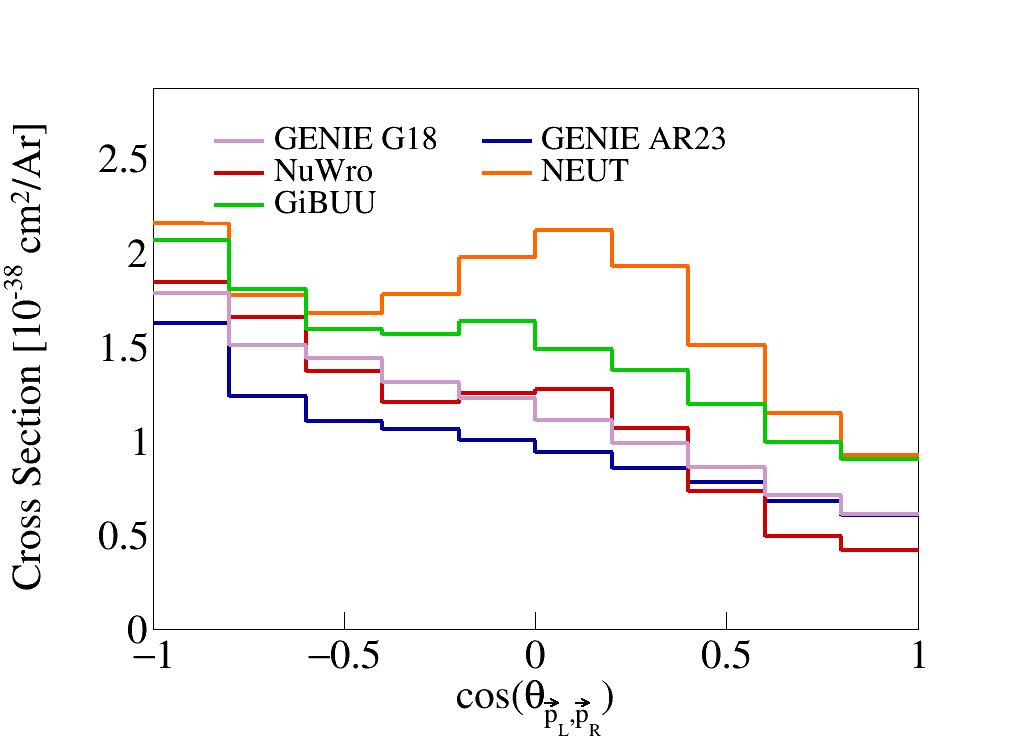
\includegraphics[width=3in]{Figs/Overlay/Overlay_TrueCosOpeningAngleProtonsPlot.png}}
    \subfloat{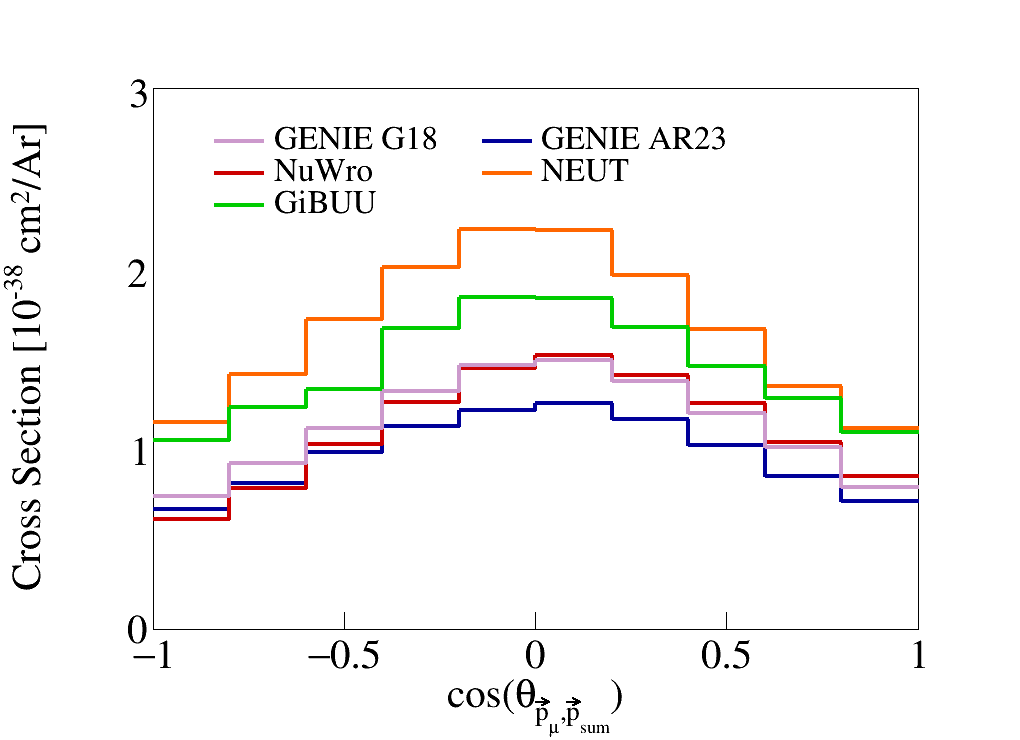
\includegraphics[width=3in]{Figs/Overlay/Overlay_TrueCosOpeningAngleMuonTotalProtonPlot.png}} \\
    \subfloat{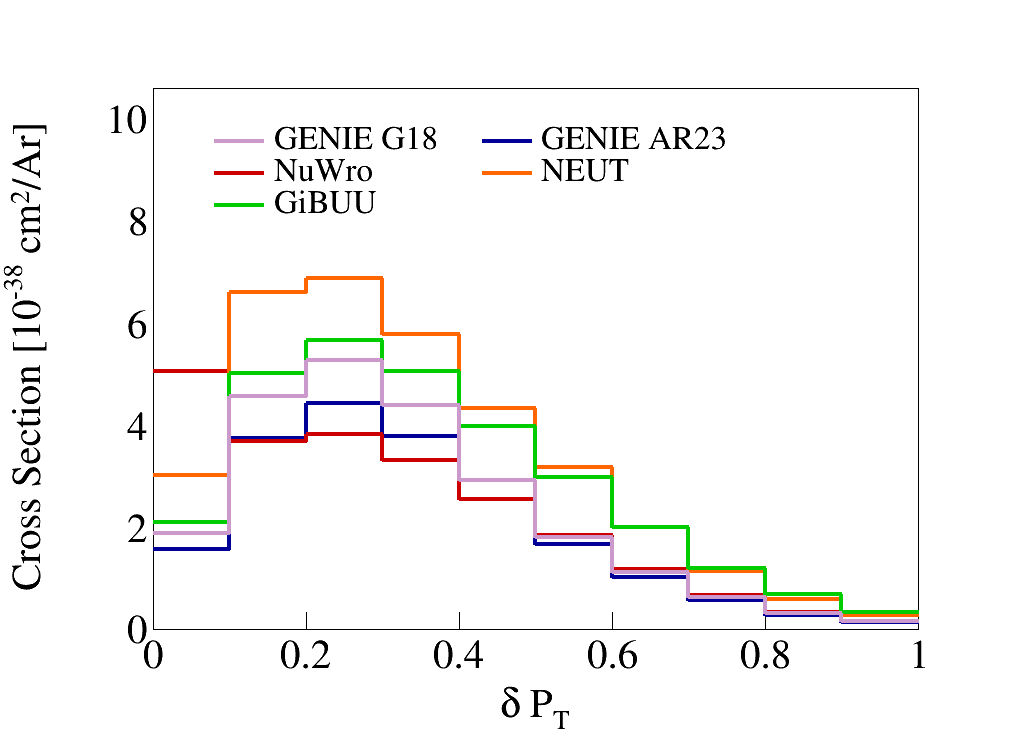
\includegraphics[width=3in]{Figs/Overlay/Overlay_TrueTransverseMomentumPlot.png}}
    \caption{Differential cross sections for opening angles and transverse momentum.}
    \label{fig:angles-transverse-momentum}
\end{figure}

\begin{figure}[H]
    \centering
    \subfloat{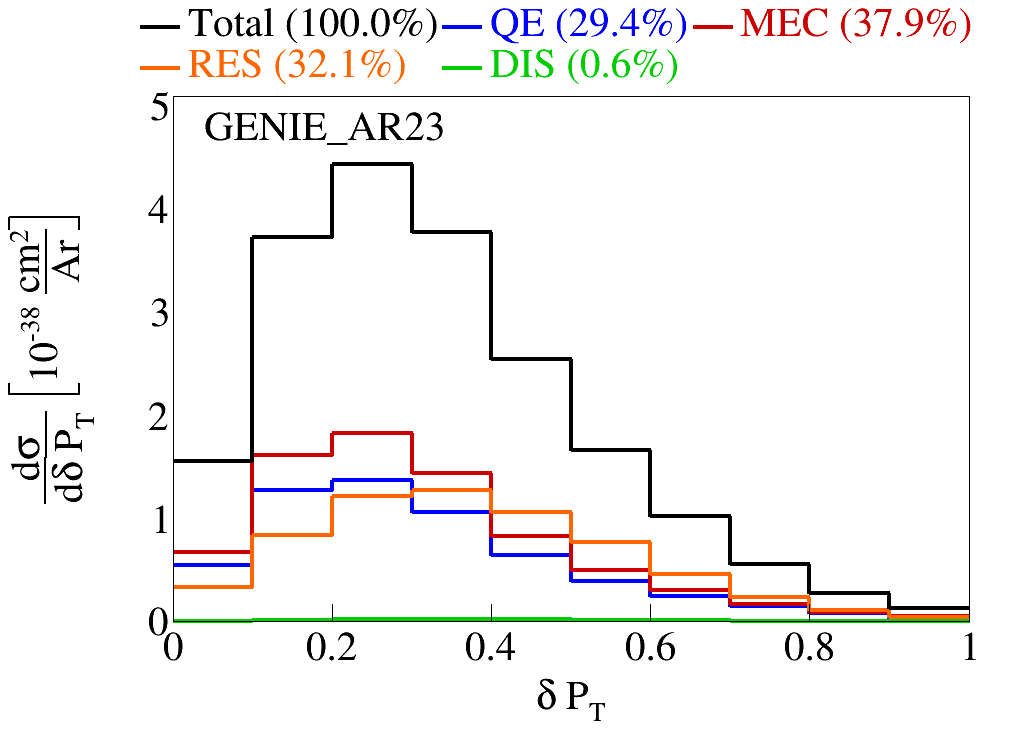
\includegraphics[width=3in]{Figs/InteBreakDown/InteBreakDown_GENIE_AR23_TrueTransverseMomentumPlot.png}}
    \subfloat{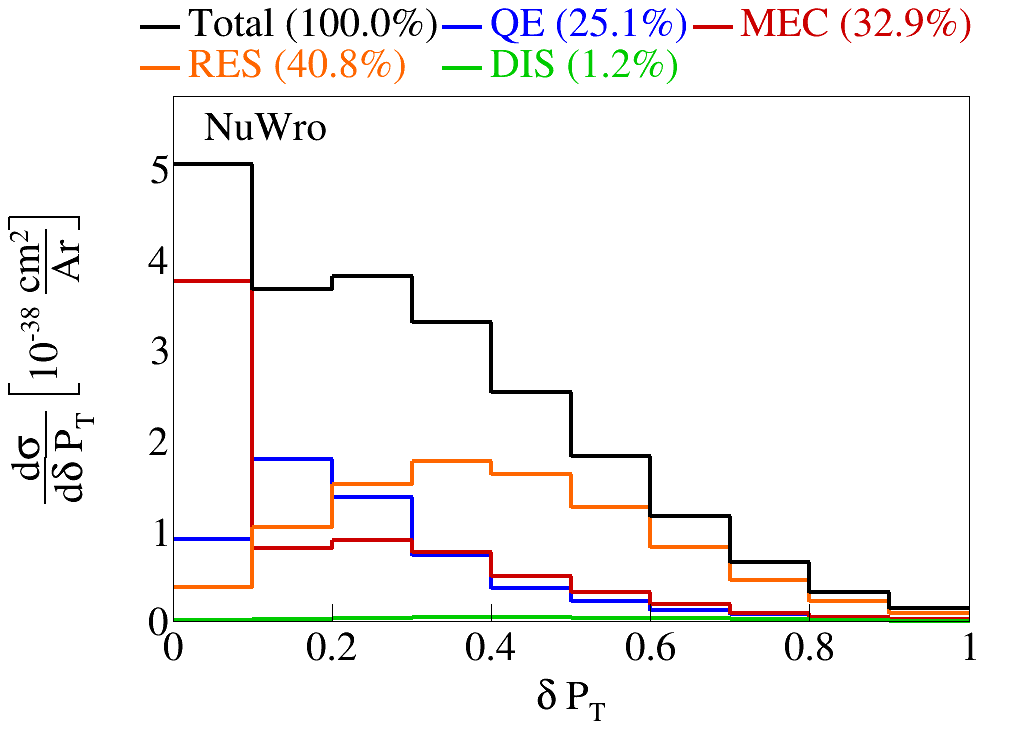
\includegraphics[width=3in]{Figs/InteBreakDown/InteBreakDown_NuWro_TrueTransverseMomentumPlot.png}}
    \caption{Event interaction breakdown for $|\vdp|$.}
    \label{fig:inte-breakdown-dpt}
\end{figure}


\end{document}
